\section{Лекція 1: Основні терміни. \label{chap1}}

У підготовці інженерів-електромеханіків задіяні чотири галузі інженерії: механічна та електрична інженерія (спільним ядром яких і є електромеханіка), електронна інженерія та автоматизація. Спільне використання теорії, методів та засобів цих галузей приводить до виникнення комбінованої галузі інженерії - мехатроніки.

\begin{figure}[h!]
	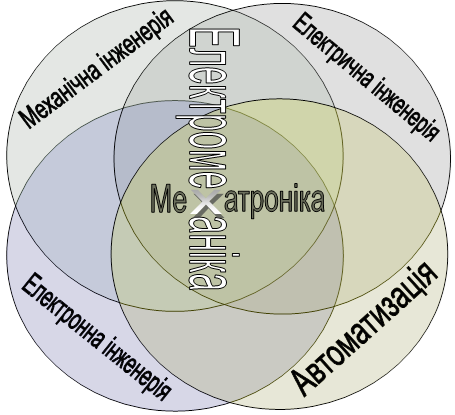
\includegraphics{Fig1.png}
	\centering
	\caption{Мехатроніка як комбінована галузь інженерії.}
\end{figure}